\documentclass[11pt,a4paper]{report}
\usepackage[textwidth=37em,vmargin=30mm]{geometry}
\usepackage{calc,xunicode,amsmath,amssymb,paralist,enumitem,tabu,booktabs,datetime2,xeCJK,xeCJKfntef,listings}
\usepackage{tocloft,fancyhdr,tcolorbox,xcolor,graphicx,eso-pic,xltxtra,xelatexemoji}

\newcommand{\envyear}[0]{2025}
\newcommand{\envdatestr}[0]{2025-02-07}
\newcommand{\envfinaldir}[0]{webdb/2025/20250207/final}

\usepackage[hidelinks]{hyperref}
\hypersetup{
    colorlinks=false,
    pdfpagemode=FullScreen,
    pdftitle={Web Digest - \envdatestr}
}

\setlength{\cftbeforechapskip}{10pt}
\renewcommand{\cftchapfont}{\rmfamily\bfseries\large\raggedright}
\setlength{\cftbeforesecskip}{2pt}
\renewcommand{\cftsecfont}{\sffamily\small\raggedright}

\setdefaultleftmargin{2em}{2em}{1em}{1em}{1em}{1em}

\usepackage{xeCJK,xeCJKfntef}
\xeCJKsetup{PunctStyle=plain,RubberPunctSkip=false,CJKglue=\strut\hskip 0pt plus 0.1em minus 0.05em,CJKecglue=\strut\hskip 0.22em plus 0.2em}
\XeTeXlinebreaklocale "zh"
\XeTeXlinebreakskip = 0pt


\setmainfont{Brygada 1918}
\setromanfont{Brygada 1918}
\setsansfont{IBM Plex Sans}
\setmonofont{JetBrains Mono NL}
\setCJKmainfont{Noto Serif CJK SC}
\setCJKromanfont{Noto Serif CJK SC}
\setCJKsansfont{Noto Sans CJK SC}
\setCJKmonofont{Noto Sans CJK SC}

\setlength{\parindent}{0pt}
\setlength{\parskip}{8pt}
\linespread{1.15}

\lstset{
	basicstyle=\ttfamily\footnotesize,
	numbersep=5pt,
	backgroundcolor=\color{black!5},
	showspaces=false,
	showstringspaces=false,
	showtabs=false,
	tabsize=2,
	captionpos=b,
	breaklines=true,
	breakatwhitespace=true,
	breakautoindent=true,
	linewidth=\textwidth
}






\newcommand{\coverpic}[2]{
    % argv: itemurl, authorname
    Cover photo by #2~~(\href{#1}{#1})
}
\newcommand{\makeheader}[0]{
    \begin{titlepage}
        % \newgeometry{hmargin=15mm,tmargin=21mm,bmargin=12mm}
        \begin{center}
            
            \rmfamily\scshape
            \fontspec{BaskervilleF}
            \fontspec{Old Standard}
            \fontsize{59pt}{70pt}\selectfont
            WEB\hfill DIGEST
            
            \vfill
            % \vskip 30pt
            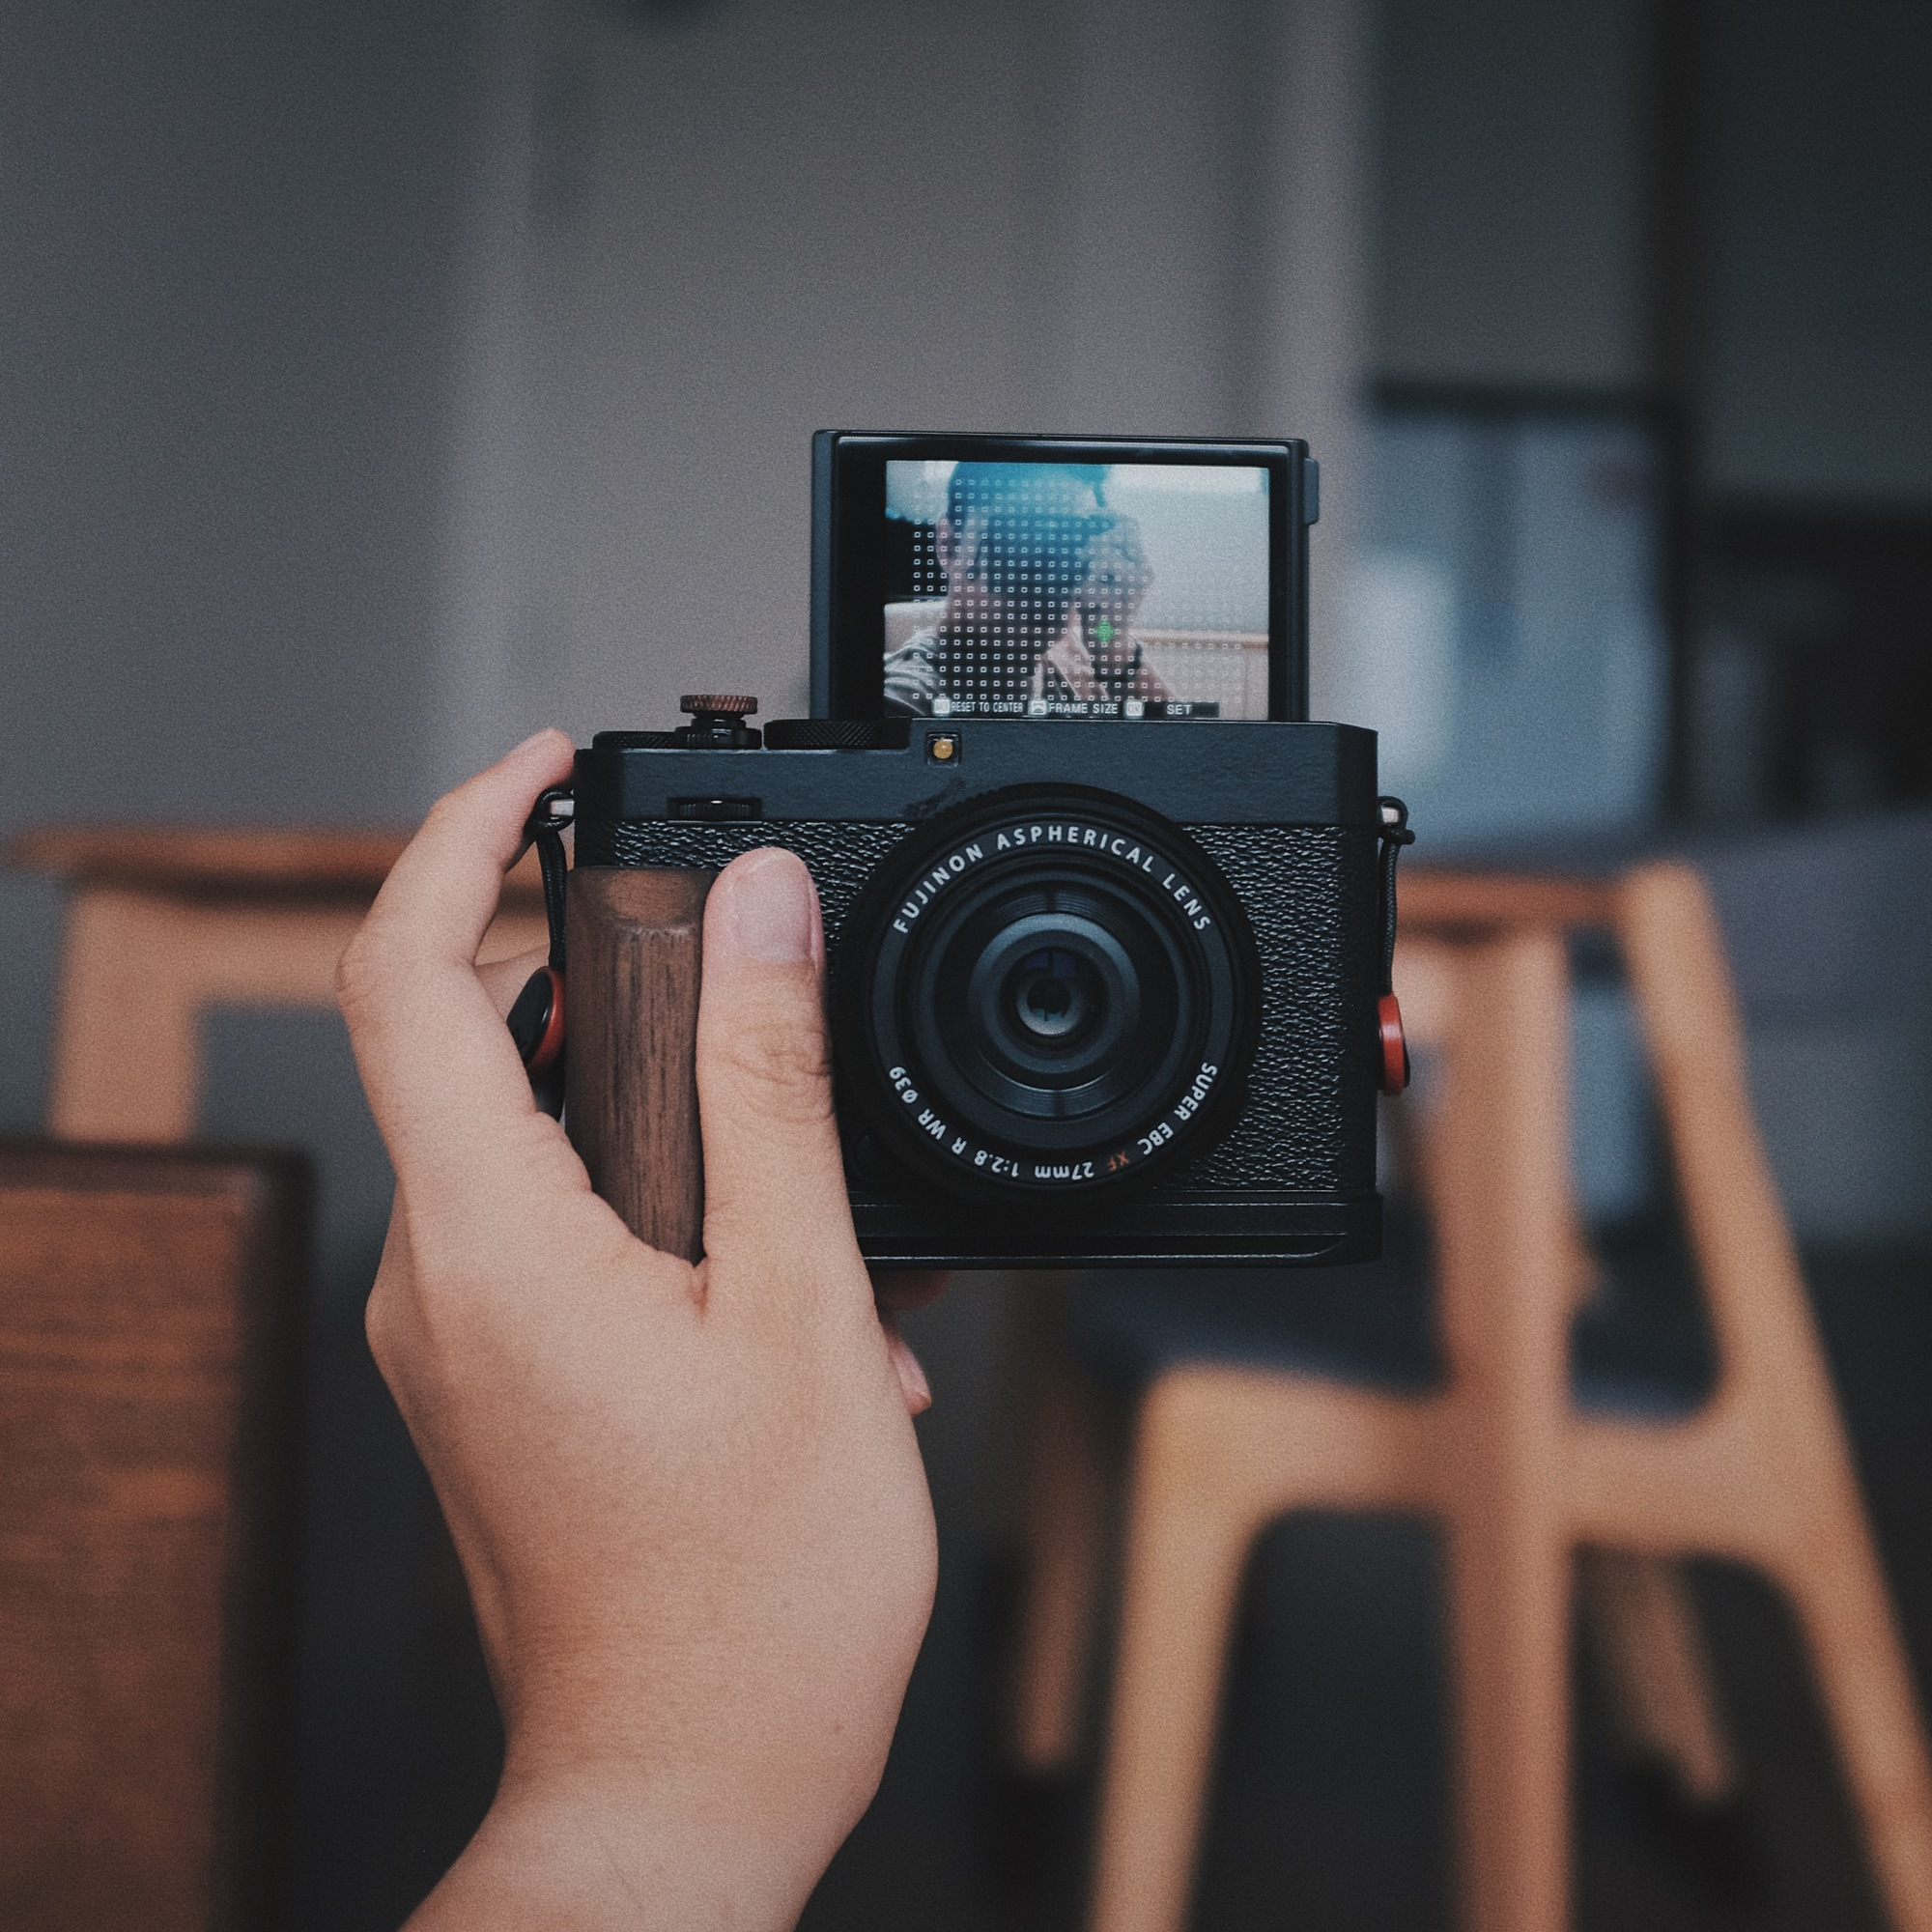
\includegraphics[width=\linewidth]{\envfinaldir/coverpic-prod.jpg}\par
            % \vskip 30pt
            \vfill

            \normalsize\rmfamily\scshape
            \copyright{} The Web Digest Project \hfill\large \envdatestr
        \end{center}
    \end{titlepage}
    % \restoregeometry
}
\newcommand{\simplehref}[1]{%
    \textcolor{blue!80!green}{\href{#1}{#1}}%
}
\renewcommand{\contentsname}{\center\Huge\sffamily\bfseries Contents\par\vskip 20pt}
\newcounter{ipartcounter}
\setcounter{ipartcounter}{0}
\newcommand{\ipart}[1]{
    % \vskip 20pt
    \clearpage
    \stepcounter{ipartcounter}
    \phantomsection
    \addcontentsline{toc}{chapter}{#1}
    % \begin{center}
    %     \Huge
    %     \sffamily\bfseries
    %     #1
    % \end{center}
    % \vskip 20pt plus 7pt
}
\newcounter{ichaptercounter}
\setcounter{ichaptercounter}{0}
\newcommand{\ichapter}[1]{
    % \vskip 20pt
    \clearpage
    \stepcounter{ichaptercounter}
    \phantomsection
    \addcontentsline{toc}{section}{\numberline{\arabic{ichaptercounter}}#1}
    \begin{center}
        \Huge
        \sffamily\bfseries
        #1
    \end{center}
    \vskip 20pt plus 7pt
}
\newcommand{\entrytitlefont}[1]{\subsection*{\raggedright\Large\sffamily\bfseries#1}}
\newcommand{\entryitemGeneric}[2]{
    % argv: title, url
    \parbox{\linewidth}{
        \entrytitlefont{#1}\par\vskip 5pt
        \footnotesize\ttfamily\mdseries
        \simplehref{#2}
    }\vskip 11pt plus 11pt minus 1pt
}
\newcommand{\entryitemGithub}[3]{
    % argv: title, url, desc
    \parbox{\linewidth}{
        \entrytitlefont{#1}\par\vskip 5pt
        \footnotesize\ttfamily\mdseries
        \simplehref{#2}\par\vskip 5pt
        \small\rmfamily\mdseries#3
    }\vskip 11pt plus 11pt minus 1pt
}
\newcommand{\entryitemAp}[3]{
    % argv: title, url, desc
    \parbox{\linewidth}{
        \entrytitlefont{#1}\par\vskip 5pt
        \footnotesize\ttfamily\mdseries
        \simplehref{#2}\par\vskip 5pt
        \small\rmfamily\mdseries#3
    }\vskip 11pt plus 11pt minus 1pt
}
\newcommand{\entryitemHackernews}[3]{
    % argv: title, hnurl, rawurl
    % \parbox{\linewidth}{
    %     \entrytitlefont{#1}\par\vskip 5pt
    %     \footnotesize\ttfamily\mdseries
    %     \simplehref{#3}\par
    %     \textcolor{black!50}{\href{#2}{#2}}
    % }\vskip 11pt plus 11pt minus 1pt
    \begin{minipage}{\linewidth}
            \entrytitlefont{#1}\par\vskip 5pt
            \footnotesize\ttfamily\mdseries
            \simplehref{#3}\par
            \textcolor{black!50}{\href{#2}{#2}}
    \end{minipage}\par\vskip 11pt plus 11pt minus 1pt
}







\begin{document}

\makeheader

\tableofcontents\clearpage




\ipart{Developers}
\ichapter{Hacker News}
\entryitemTwoLinks{R1 Computer Use}{https://news.ycombinator.com/item?id=42965954}{https://github.com/agentsea/r1-computer-use}

\entryitemTwoLinks{Show HN: SQLite disk page explorer}{https://news.ycombinator.com/item?id=42965198}{https://github.com/QuadrupleA/sqlite-page-explorer}

\entryitemTwoLinks{Scala 3 Migration: Report from the field}{https://news.ycombinator.com/item?id=42964773}{https://blog.pierre-ricadat.com/scala-3-migration-report-from-the-field}

\entryitemTwoLinks{GitHub Copilot: The Agent Awakens}{https://news.ycombinator.com/item?id=42964327}{https://github.blog/news-insights/product-news/github-copilot-the-agent-awakens/}

\entryitemTwoLinks{Show HN: An homage to Tom Dowdy's 1991 screensaver, "Kaos"}{https://news.ycombinator.com/item?id=42963346}{https://thestrikeagency.com/kaos/}

\entryitemTwoLinks{U.S. Government Disclosed 39 Zero-Day Vulnerabilities in 2023, First-Ever Report}{https://news.ycombinator.com/item?id=42962702}{https://www.zetter-zeroday.com/u-s-government-disclosed-39-zero-day-vulnerabilities-in-2023-per-first-ever-report/}

\entryitemTwoLinks{Simulating water over terrain}{https://news.ycombinator.com/item?id=42962508}{https://lisyarus.github.io/blog/posts/simulating-water-over-terrain.html}

\entryitemTwoLinks{Pre-Trained Large Language Models Use Fourier Features for Addition (2024)}{https://news.ycombinator.com/item?id=42960989}{https://arxiv.org/abs/2406.03445}

\entryitemTwoLinks{Aluminum Batteries Outlive Lithium-Ion with a Pinch of Salt}{https://news.ycombinator.com/item?id=42960907}{https://spectrum.ieee.org/aluminum-battery}

\entryitemTwoLinks{US Cloud soon illegal in EU? US punches first hole in EU-US Data Deal}{https://news.ycombinator.com/item?id=42960788}{https://noyb.eu/en/us-cloud-soon-illegal-trump-punches-first-hole-eu-us-data-deal}

\entryitemTwoLinks{Cloudflare R2 Global Outage}{https://news.ycombinator.com/item?id=42960291}{https://www.cloudflarestatus.com}

\entryitemTwoLinks{Paper Apps}{https://news.ycombinator.com/item?id=42960144}{https://gladdendesign.com/collections/paper-apps}

\entryitemTwoLinks{Linux Running in a PDF}{https://news.ycombinator.com/item?id=42959775}{https://linux.doompdf.dev/linux.pdf}

\entryitemTwoLinks{America's Dangerous Movement Toward Oligarchy, Authoritarianism and Kleptocracy}{https://news.ycombinator.com/item?id=42959260}{https://www.counterpunch.org/2025/02/04/americas-dangerous-movement-toward-oligarchy-authoritarianism-and-kleptocracy/}

\entryitemTwoLinks{Programming SDF animations of Rick and Morty}{https://news.ycombinator.com/item?id=42958696}{https://danielchasehooper.com/posts/code-animated-rick/}

\entryitemTwoLinks{Subway crime plummets as ridership jumps significantly in congestion pricing era}{https://news.ycombinator.com/item?id=42958474}{https://www.amny.com/nyc-transit/nyc-subway-crime-plummets-ridership-jumps-2025/}

\entryitemTwoLinks{Mystery brain disease patients in New Brunswick say they welcome investigation}{https://news.ycombinator.com/item?id=42958218}{https://www.ctvnews.ca/atlantic/new-brunswick/article/good-first-step-nb-mystery-brain-disease-patients-welcome-new-investigation/}

\entryitemTwoLinks{OpenWrt 24.10.0 – First Stable Release}{https://news.ycombinator.com/item?id=42958202}{https://openwrt.org/releases/24.10/notes-24.10.0}

\entryitemTwoLinks{Deep Reinforcement Learning: Pong from Pixels (2016)}{https://news.ycombinator.com/item?id=42958012}{http://karpathy.github.io/2016/05/31/rl/}

\entryitemTwoLinks{I believe 6502 instruction set is a good first assembly language}{https://news.ycombinator.com/item?id=42957823}{https://nemanjatrifunovic.substack.com/p/6502-is-a-good-starting-point-for}\ichapter{Phoronix}
\entryitemGeneric{\hskip 0pt{}VirtIO Media Driver Upstreaming Pursued For Relaying V4L2 Media Devices To Guests}{https://www.phoronix.com/news/VirtIO-Media-Driver-Patches}

\entryitemGeneric{\hskip 0pt{}SMT Remains Very Advantageous For 5th Gen AMD EPYC Performance}{https://www.phoronix.com/review/amd-epyc-zen5-smt}

\entryitemGeneric{\hskip 0pt{}AMD Talks Up IREE/MLIR Programming For Ryzen AI NPUs}{https://www.phoronix.com/news/AMD-Ryzen-AI-LLVM-MLIR-Coding}

\entryitemGeneric{\hskip 0pt{}Intel's OpenVINO 2025.0 Brings Support For Deepseek Models, Better AI Performance}{https://www.phoronix.com/news/Intel-OpenVINO-2025.0}

\entryitemGeneric{\hskip 0pt{}LibreOffice 25.2 Open-Source Office Suite Released With Many Improvements}{https://www.phoronix.com/news/LibreOffice-25.2-Released}

\entryitemGeneric{\hskip 0pt{}Mesa 25.0 Is Trending Well For Release Later This Month}{https://www.phoronix.com/news/Mesa-25.0-Trending-February}

\entryitemGeneric{\hskip 0pt{}GNU Gold Linker Is Deprecated \& Will Be Gone For Good Without New Developers}{https://www.phoronix.com/news/GNU-Gold-Linker-Deprecated}

\entryitemGeneric{\hskip 0pt{}PipeWire Is Doing An Excellent Job Handling Audio/Video Streams On The Linux Desktop}{https://www.phoronix.com/news/PipeWire-State-2025}

\entryitemGeneric{\hskip 0pt{}Google Interested In The Modern Intel Xe Linux Kernel Driver On Alder Lake}{https://www.phoronix.com/news/Google-Xe-Driver-For-Alder-Lake}\ichapter{Dribbble}
\entryitemGeneric{\hskip 0pt{}Cloaked Logo Design}{https://dribbble.com/shots/25585116-Cloaked-Logo-Design}

\entryitemGeneric{\hskip 0pt{}Carbon Solutions B2B Branding Design \& Visual Identity}{https://dribbble.com/shots/25525140-Carbon-Solutions-B2B-Branding-Design-Visual-Identity}

\entryitemGeneric{\hskip 0pt{}Dog / Puzzle Logo}{https://dribbble.com/shots/25581316-Dog-Puzzle-Logo}

\entryitemGeneric{\hskip 0pt{}Frank's Alley® Trailer \& Mascots}{https://dribbble.com/shots/25585516-Frank-s-Alley-Trailer-Mascots}

\entryitemGeneric{\hskip 0pt{}Glyph Beer Icons 51-62}{https://dribbble.com/shots/25585199-Glyph-Beer-Icons-51-62}

\entryitemGeneric{\hskip 0pt{}Realtree® 30 Years.}{https://dribbble.com/shots/25579343-Realtree-30-Years}

\entryitemGeneric{\hskip 0pt{}VCC Logo Design Vector Sketches}{https://dribbble.com/shots/25577220-VCC-Logo-Design-Vector-Sketches}

\entryitemGeneric{\hskip 0pt{}Brand Family System Loop}{https://dribbble.com/shots/25579103-Brand-Family-System-Loop}

\entryitemGeneric{\hskip 0pt{}Weve Branding}{https://dribbble.com/shots/25579635-Weve-Branding}

\entryitemGeneric{\hskip 0pt{}Chilbot Motion Design}{https://dribbble.com/shots/25578623-Chilbot-Motion-Design}

\entryitemGeneric{\hskip 0pt{}S}{https://dribbble.com/shots/25571540-S}

\entryitemGeneric{\hskip 0pt{}Fly Fry}{https://dribbble.com/shots/25573635-Fly-Fry}

\entryitemGeneric{\hskip 0pt{}Logo and Branding for VCC}{https://dribbble.com/shots/25571598-Logo-and-Branding-for-VCC}

\entryitemGeneric{\hskip 0pt{}Axolotl Mascot}{https://dribbble.com/shots/25572670-Axolotl-Mascot}

\entryitemGeneric{\hskip 0pt{}Finance APP UI Design}{https://dribbble.com/shots/25570740-Finance-APP-UI-Design}

\entryitemGeneric{\hskip 0pt{}TIAA Duotone Icons}{https://dribbble.com/shots/25573874-TIAA-Duotone-Icons}

\entryitemGeneric{\hskip 0pt{}Cloud Animation Sound Design}{https://dribbble.com/shots/25571319-Cloud-Animation-Sound-Design}

\entryitemGeneric{\hskip 0pt{}Year of the Snake}{https://dribbble.com/shots/25563617-Year-of-the-Snake}

\entryitemGeneric{\hskip 0pt{}Atlantic Pickleball Club}{https://dribbble.com/shots/25558009-Atlantic-Pickleball-Club}

\entryitemGeneric{\hskip 0pt{}Wizard Logo}{https://dribbble.com/shots/25559490-Wizard-Logo}

\entryitemGeneric{\hskip 0pt{}Stellar}{https://dribbble.com/shots/25559656-Stellar}

\entryitemGeneric{\hskip 0pt{}VCC Final Logo Animation}{https://dribbble.com/shots/25557794-VCC-Final-Logo-Animation}

\entryitemGeneric{\hskip 0pt{}Saturday Quiz Time Icons}{https://dribbble.com/shots/25561868-Saturday-Quiz-Time-Icons}

\entryitemGeneric{\hskip 0pt{}Crypto onboarding illustrations}{https://dribbble.com/shots/25555520-Crypto-onboarding-illustrations}


\ipart{Developers~~~~(zh-Hans)}
\ichapter{Solidot}
\entryitemGeneric{\hskip 0pt{}苹果面临反垄断调查}{https://www.solidot.org/story?sid=80487}

\entryitemGeneric{\hskip 0pt{}OpenWrt 24.10 释出}{https://www.solidot.org/story?sid=80486}

\entryitemGeneric{\hskip 0pt{}iPhone 在华销量大幅下挫}{https://www.solidot.org/story?sid=80485}

\entryitemGeneric{\hskip 0pt{}本田与日产合并谈判破裂}{https://www.solidot.org/story?sid=80484}

\entryitemGeneric{\hskip 0pt{}DeepSeek 使用了中移动的基础设施}{https://www.solidot.org/story?sid=80483}

\entryitemGeneric{\hskip 0pt{}研究称早上幸福感最高}{https://www.solidot.org/story?sid=80482}

\entryitemGeneric{\hskip 0pt{}美国冻结对外援助打击全世界的研究项目}{https://www.solidot.org/story?sid=80481}

\entryitemGeneric{\hskip 0pt{}AMD 数据中心收入首次超过英特尔}{https://www.solidot.org/story?sid=80480}

\entryitemGeneric{\hskip 0pt{}F-Droid 项目获得约 40 万美元拨款}{https://www.solidot.org/story?sid=80479}

\entryitemGeneric{\hskip 0pt{}泰国对妙瓦底等缅甸地区断电断网}{https://www.solidot.org/story?sid=80478}

\entryitemGeneric{\hskip 0pt{}DeepSeek 研究称华为昇腾 910C 推理性能能达到英伟达 H100 的六成}{https://www.solidot.org/story?sid=80477}

\entryitemGeneric{\hskip 0pt{}AI 生成内容进入了公共图书馆}{https://www.solidot.org/story?sid=80476}

\entryitemGeneric{\hskip 0pt{}天文学家在系外行星上发现风速高达 9 公里/秒的超音速气流}{https://www.solidot.org/story?sid=80475}

\entryitemGeneric{\hskip 0pt{}Paragon 证实美国及其盟国是其客户}{https://www.solidot.org/story?sid=80474}

\entryitemGeneric{\hskip 0pt{}美国邮政停收内地和香港的包裹 }{https://www.solidot.org/story?sid=80473}

\entryitemGeneric{\hskip 0pt{}Google 更新 AI 政策移除了不将 AI 用于武器和监视的承诺}{https://www.solidot.org/story?sid=80472}

\entryitemGeneric{\hskip 0pt{}波兰逮捕批准购买间谍软件 Pegasus 的前司法部长}{https://www.solidot.org/story?sid=80471}

\entryitemGeneric{\hskip 0pt{}FSF 将在下月拍卖纪念品}{https://www.solidot.org/story?sid=80470}

\entryitemGeneric{\hskip 0pt{}Framework 推出售价 199 美元的 RISC-V 主板}{https://www.solidot.org/story?sid=80469}

\entryitemGeneric{\hskip 0pt{}工商总局对谷歌发起反垄断调查}{https://www.solidot.org/story?sid=80468}\ichapter{V2EX}
\entryitemGeneric{\hskip 0pt{}[分享创造] [出海收款]Paddle 账户申请保姆级教程}{https://www.v2ex.com/t/1109485}

\entryitemGeneric{\hskip 0pt{}[分享创造] Python 和木兰报错信息对应例程整理(一)}{https://www.v2ex.com/t/1109484}

\entryitemGeneric{\hskip 0pt{}[汽车] 关于后车快速接近,应不应该变道,我建议不要变道}{https://www.v2ex.com/t/1109483}

\entryitemGeneric{\hskip 0pt{}[健康] 感染甲流之后胸口疼,不知道有没有相同情况的}{https://www.v2ex.com/t/1109482}

\entryitemGeneric{\hskip 0pt{}[Windows] WSL2 会在后台自动更新并且直接强制停止?}{https://www.v2ex.com/t/1109481}

\entryitemGeneric{\hskip 0pt{}[生活] 老家没人了,过年你还回去吗?}{https://www.v2ex.com/t/1109480}

\entryitemGeneric{\hskip 0pt{}[投资] 假设你现在有 100w 做投资,你会如何分配?投资什么?}{https://www.v2ex.com/t/1109479}

\entryitemGeneric{\hskip 0pt{}[问与答] 阅读障碍,求一款 epub 文字转语音的软件}{https://www.v2ex.com/t/1109478}

\entryitemGeneric{\hskip 0pt{}[分享发现] 回家过年/高速应该怎么开? 10 年实际驾龄老司机首次出主动事故 的 拙见分享}{https://www.v2ex.com/t/1109477}

\entryitemGeneric{\hskip 0pt{}[iOS] iOS 上有什么软件可以限制孩子使用设备的 app?}{https://www.v2ex.com/t/1109475}

\entryitemGeneric{\hskip 0pt{}[Flutter] Flutter 开发桌面应用程序,如何获取鼠标的绝对坐标?}{https://www.v2ex.com/t/1109474}

\entryitemGeneric{\hskip 0pt{}[投资] 2025 年了,求稳定年化 4\%方案}{https://www.v2ex.com/t/1109473}

\entryitemGeneric{\hskip 0pt{}[汽车] 求购一辆甲壳虫三代,预算 5w 左右}{https://www.v2ex.com/t/1109472}

\entryitemGeneric{\hskip 0pt{}[问与答] 请问 v 站发帖现在是有话题限制吗?}{https://www.v2ex.com/t/1109471}

\entryitemGeneric{\hskip 0pt{}[宽带症候群] mihomo 是否存在这种配置(所有流量,先走一个 SOCKS5)}{https://www.v2ex.com/t/1109470}

\entryitemGeneric{\hskip 0pt{}[Apple] Apple Intelligence GPT 登录后自动降级成 Free}{https://www.v2ex.com/t/1109469}

\entryitemGeneric{\hskip 0pt{}[问与答] 请教各位,太阳能储电相关.}{https://www.v2ex.com/t/1109467}

\entryitemGeneric{\hskip 0pt{}[问与答] 有类似 Wrap 的终端推荐吗?}{https://www.v2ex.com/t/1109465}

\entryitemGeneric{\hskip 0pt{}[游戏] 分享一下我对 DLSS 的看法}{https://www.v2ex.com/t/1109464}

\entryitemGeneric{\hskip 0pt{}[全球工单系统] Cloudflare 巴西地区服务故障}{https://www.v2ex.com/t/1109463}

\entryitemGeneric{\hskip 0pt{}[生活] 舍友嫌弃我打呼噜 搬去其他宿舍了,个人 BMI:21 不到}{https://www.v2ex.com/t/1109462}

\entryitemGeneric{\hskip 0pt{}[酷工作] [代发] Python 桌面软件开发工程师或项目团队招聘(全职)}{https://www.v2ex.com/t/1109457}

\entryitemGeneric{\hskip 0pt{}[问与答] cursor 骚操作,说说话为 GA4 添加自定义分析代码}{https://www.v2ex.com/t/1109456}

\entryitemGeneric{\hskip 0pt{}[程序员] Deepseek R1 671B 本地部署计算机硬件配置?}{https://www.v2ex.com/t/1109455}

\entryitemGeneric{\hskip 0pt{}[程序员] Cursor 是无法处理多项目的工作区吗?大家怎么做?}{https://www.v2ex.com/t/1109454}

\entryitemGeneric{\hskip 0pt{}[问与答] 大家不踩雷的 1688 床笠被罩等家纺店铺可以推荐一下吗}{https://www.v2ex.com/t/1109452}

\entryitemGeneric{\hskip 0pt{}[问与答] 求推荐一个应用可以将音频文件转成文本}{https://www.v2ex.com/t/1109451}

\entryitemGeneric{\hskip 0pt{}[分享创造] 写了个饥荒食谱速查工具}{https://www.v2ex.com/t/1109450}

\entryitemGeneric{\hskip 0pt{}[分享发现] 悲伤,欧版 s25u 不支持电信或者移动 5g。联通没试。。。}{https://www.v2ex.com/t/1109449}

\entryitemGeneric{\hskip 0pt{}[程序员] 哪些大佬有工具导航站啊?我想付费提交一下我的工具站}{https://www.v2ex.com/t/1109448}

\entryitemGeneric{\hskip 0pt{}[罗技] MX Master 3s 在 macOS 上时不时卡顿}{https://www.v2ex.com/t/1109447}

\entryitemGeneric{\hskip 0pt{}[Google] YouTube Analytics API 的每日配额怎么申请提额?有偿}{https://www.v2ex.com/t/1109445}

\entryitemGeneric{\hskip 0pt{}[问与答] 公积金有必要提前还款吗?}{https://www.v2ex.com/t/1109444}

\entryitemGeneric{\hskip 0pt{}[macOS] 更新 macOS15 和 iOS18 后使用 VPN Safari 无法打开 http 网页,关掉不受影响?大家有这种情况吗?}{https://www.v2ex.com/t/1109443}

\entryitemGeneric{\hskip 0pt{}[问与答] 大佬们有什么前端面试范文推荐的吗}{https://www.v2ex.com/t/1109441}

\entryitemGeneric{\hskip 0pt{}[分享创造] 24 小时前端零基础用 Windsurf + Claude 上线一个简单的工具类网页}{https://www.v2ex.com/t/1109440}

\entryitemGeneric{\hskip 0pt{}[分享创造] 「软件限免」信息共建共享方案}{https://www.v2ex.com/t/1109439}

\entryitemGeneric{\hskip 0pt{}[程序员] 分享一下以太坊 Protocol Wiki 中文版}{https://www.v2ex.com/t/1109435}

\entryitemGeneric{\hskip 0pt{}[Windows] Win 11 的中英文输入切换突然变成按两下 shift 键了?}{https://www.v2ex.com/t/1109434}

\entryitemGeneric{\hskip 0pt{}[问与答] 硅基流动部署的 deepseek}{https://www.v2ex.com/t/1109433}

\entryitemGeneric{\hskip 0pt{}[推广] AI 心理测试 淘宝新店``零元购'' MBTI 抑郁焦虑 性格人格测试 AI 生成解读报告}{https://www.v2ex.com/t/1109432}

\entryitemGeneric{\hskip 0pt{}[Android] android 版 wine 只更新到 7.0 版,安装时提示 sdk 版本过低,有替代方案吗?}{https://www.v2ex.com/t/1109430}

\entryitemGeneric{\hskip 0pt{}[程序员] [AI] 为啥现在一边喊着 AI 代替人类,另一边各种场景 AI 落地却困难重重}{https://www.v2ex.com/t/1109429}

\entryitemGeneric{\hskip 0pt{}[RSS] Follow 貌似会丢失历史未看的文章}{https://www.v2ex.com/t/1109428}

\entryitemGeneric{\hskip 0pt{}[问与答] macos ifconfig 这几个网路接口是什么,导致注册到 nacos 是它,不是 en0 无法与其他人交互}{https://www.v2ex.com/t/1109427}

\entryitemGeneric{\hskip 0pt{}[生活] 有感于 v 友的帖子,说说我的肠胃,祝大家健康}{https://www.v2ex.com/t/1109426}

\entryitemGeneric{\hskip 0pt{}[分享发现] 爽!年前遇到一辆马路当自家客厅的理想,直接给这哥们来了个大满贯套餐。}{https://www.v2ex.com/t/1109425}

\entryitemGeneric{\hskip 0pt{}[分享创造] [油猴脚本] 强制所有链接在新标签页打开}{https://www.v2ex.com/t/1109424}

\entryitemGeneric{\hskip 0pt{}[酷工作] [深圳] 科技创新企业 [至简天成] 招聘 高级前端开发工程师(AI 方向)2 人 - 25 年春招启动了}{https://www.v2ex.com/t/1109423}

\entryitemGeneric{\hskip 0pt{}[分享发现] DeepSeek 初体验}{https://www.v2ex.com/t/1109421}


\ipart{Generic News}
\ichapter{AP News}
\entryitemWithDescription{\hskip 0pt{}`SNL50' anniversary special will feature Bad Bunny, Sabrina Carpenter, Dave Chappelle and more}{https://apnews.com/article/1688704b7bb07bbd01802fee9138ff26}{}

\entryitemWithDescription{\hskip 0pt{}Telescopes spy a monster radio jet streaming from a bright and early object in the universe}{https://apnews.com/article/0822cd50b4f39c5902146c1ea893a76f}{}

\entryitemWithDescription{\hskip 0pt{}Winter storms bring flooding and `thunder ice' in several US states}{https://apnews.com/article/df985dd578a891b0e2fd33482170f21f}{}

\entryitemWithDescription{\hskip 0pt{}Irv Gotti, music executive who created Murder Inc. Records, dies at 54}{https://apnews.com/article/745f00b1b0c024916d874f6bbf123355}{}

\entryitemWithDescription{\hskip 0pt{}Honeywell, one of the few remaining US industrial conglomerates, will split into three companies}{https://apnews.com/article/24e46c1e34bfeb702acecead3fd98060}{}

\entryitemWithDescription{\hskip 0pt{}Kansas City Chiefs player becomes a coach to a mutt named Parsnip for the `Puppy Bowl'}{https://apnews.com/article/0d3a65750c94ca476c59b47a564b3ebf}{}

\entryitemWithDescription{\hskip 0pt{}Freezing hikers stuck in waist-deep snow rescued during Mount Washington whiteout}{https://apnews.com/article/0f5fa5d1cf442e22caa0beecd9ec766a}{}

\entryitemWithDescription{\hskip 0pt{}Baseball star Ohtani's ex-interpreter to appear in court for sentencing in betting case}{https://apnews.com/article/3a721012444e0768eed2a1250b027e72}{}

\entryitemWithDescription{\hskip 0pt{}The heist of 100,000 eggs in Pennsylvania becomes a whodunit that police have yet to crack}{https://apnews.com/article/c1c260ca05b9f84612c61071cb504939}{}

\entryitemWithDescription{\hskip 0pt{}Boy Scouts see a small membership uptick after rebrand to Scouting America}{https://apnews.com/article/796935fe9474fda03d179aa8c087ab42}{}

\entryitemWithDescription{\hskip 0pt{}Drake and Kendrick Lamar's beef — from its beginnings to the Super Bowl — explained}{https://apnews.com/article/0f9acb354f9041bbb0e5279dea718fff}{}

\entryitemWithDescription{\hskip 0pt{}`Wicked' star Cynthia Erivo is feted as Harvard's Hasty Pudding Woman of the Year}{https://apnews.com/article/a2d4c361c9b036a04107c885b7f42946}{}

\entryitemWithDescription{\hskip 0pt{}Fox News hires president's daughter-in-law Lara Trump for weekend show on network}{https://apnews.com/article/9585f6d27cbf74942ff3e2db560bbe64}{}






\clearpage
\leavevmode\vfill
\footnotesize

Copyright \copyright{} 2023-2025 Neruthes and other contributors.

This document is published with CC BY-NC-ND 4.0 license.

The entries listed in this newsletter may be copyrighted by their respective creators.

This newsletter is generated by the Web Digest project.

The newsletters are also delivered via Telegram channel \CJKunderline{\href{https://t.me/webdigestchannel}{https://t.me/webdigestchannel}}.\\
RSS feed is available at \CJKunderline{\href{https://webdigest.pages.dev/rss.xml}{https://webdigest.pages.dev/rss.xml}}.

This newsletter is available in PDF at
\CJKunderline{\href{https://webdigest.pages.dev/}{https://webdigest.pages.dev/}}.

The source code being used to generate this newsletter is available at\\
\CJKunderline{\href{https://github.com/neruthes/webdigest}{https://github.com/neruthes/webdigest}}.

This newsletter is also available in
\CJKunderline{\href{http://webdigest.pages.dev/readhtml/\envyear/WebDigest-20250207.html}{HTML}} and
\CJKunderline{\href{https://github.com/neruthes/webdigest/blob/master/markdown/\envyear/WebDigest-20250207.md}{Markdown}}.


\coverpic{https://unsplash.com/photos/a-man-and-a-woman-holding-hands-on-a-beach--a6yt6Cy0ek}{Alexander Mass}


\end{document}
